\chapter{Grundlagen Maschinelles \\ Lernen \label{Chapter-ML}}

\section{Eingränzung}

\subsection*{Eingrenzung}

Das umfassende Feld des Maschinellen Lernens (ML) befasst sich mit vielen Bereichen;
 Die zwei prominetesten sind dabei das Supervised und Unsupervised Learning. In beiden Fällen wird eine Funktion
 $f: X \rightarrow Y$ gelernt, die aus der Menge möglicher Datenpunkte $X$ auf die Menge der zu schätzenden
 Variablen $Y$ abbildet. Hierbei besitzen die Trainingsdaten für Unsupervised ML jedoch keine Informationen für
 die Variable $y \in Y$. Dies kann beispielsweise interessant sein, wenn der Datensatz in zwei oder mehr distinkte
 Gruppen aufgeteilt werden soll, ohne dass im Vorhinein etwas über die Verteilung bekannt ist. Solch eine
 Aufgabe ist als Clustering-Aufgabe bekannt. Die Leck-Detektion benötigt jedoch weitere Informationen;
 Denn im Gegensatz zu Unsupervised ML ist beim Supervised ML diese sogenannte Ground Truth (GT) bekannt und
 das jeweilige Problem lässt sich anhand der Definition des Bildbereichs weiter eingrenzen: Die für die
 Arbeit wichtigen Arten sind hier die binäre Klassifikation und die Regression.

Bei der binären Klassifikation soll jeder Datenpunkt $x \in X$ einer von zwei Klassen $y \in \{0, 1\}$ zugewiesen
 werden. Auf unser Problem der Leck-Detektion angewendet, hieße eine Klassifikation eines Zeitpunkts in
 Klasse $1$, dass irgendwo in dem WDN ein Leck existiert, wohingegen Klasse $0$ die Abwesenheit sämtlicher
 Lecks impliziert. Für die Regression wird jedem Datenpunkt ein reeller Wert $y \in \mathbb{R}$ zugewiesen.
 Wie dieses Konzept übernommen werden kann, ist in Kapitel \ref{Chapter-Methods} weiter beschrieben. 


\subsection*{Modelle des Maschinellen Lernens}

Für jeden Anwendungsbereich gibt es eine Vielzahl an verschiedenen Algorithmen, welche eine gegebene Aufgabe
 lösen können. Die in dieser Arbeit benutzten Modelle werden im Folgenden erklärt. Hierbei ist wichtig, zwischen
 Parametern und Hyperparametern zu unterscheiden. Ersteres sind dabei die Variablen und Gewichte, die während
 des Lernprozesses optimiert oder gefunden werden. Die sogenannten Hyperparameter sind Einstellungen, welche
 vor dem Training konfiguriert werden und damit das Ergebnis erheblich verändern können.

\begin{itemize}

   \item \textbf{k-Nearest Neighbors (kNN)} ist ein einfaches Modell, bei dem ein neuer Datenpunkt nach der
    Mehrheit seiner Nachbarn $(x_i, y_i)$ in einem n-dimensionalen Koordinatensystem klassifiziert wird. Der
    Hyperparameter $k$ bestimmt hierbei, wie groß die zu betrachtende Nachbarschaft ist. Sei
            $\mathcal{N}(\hat{x}, \mathcal{D}, k)$
    die Menge der $k$ am nächsten zu $\hat{x}$ liegenden Punkte aus $\mathcal{D}$, dann ist
            $P(\hat{x}=c|\hat{x}, \mathcal{D}, k) = \frac{1}{k} |\{x_i | x_i \in \mathcal{N}(\hat{x}, \mathcal{D}, k), y_i=c\}|$
    der Anteil der Klasse $c$ in der Nachbarschaft. Die finale Klasse des neuen Datenpunktes $\hat{x}$ ist dann
    gegeben durch die am meisten vertretene Klasse:
    \begin{equation}
            f_{kNN}(\hat{x}) = \underset{c \in \{1..C\}}{\mathrm{argmax}}\ P(\hat{x}=c|\hat{x}, \mathcal{D}, k)
    \end{equation}
    Mit einem weitereren Hyperparameter lässt sich zusätzlich eine Gewichtung der Punkte hinzufügen: Anders als
    bei der oben beschriebenen uniformen Gewichtung haben bei abstandsbasierter Gewichtung die Nachbarn, die näher
    an dem zu klassifizierenden Punkt liegen einen höheren Wert im Vergleich zu Nachbarn, die weiter entfernt sind.

   \item \textbf{Multi-Layer Perceptron (MLP)} versucht, ein künstliches neuronales Netz zu erschaffen, indem es
    mehrere Perzeptronen aneinanderreiht. Ein Perzeptron steht hier für ein Neuron, welches mehrere Eingabewerte
    hat und daraus einen Ausgabewert erstellt. Dafür wird jeder Eingabewert mit einem speziell dafür gelernten
    Gewicht multipliziert und anschließend aufsummiert. Zu dieser Summe kann dann noch ein Schwellwert $\theta$
    hinzuaddiert werden, welches ebenso beim Lernen optimiert wird. Als letztes wird darauf eine sogenannte
    Aktivierungsfunktion angewendet, was dann die Ausgabe des Perzeptron bildet. Die Aktivierungsfunktionen,
    welche in dieser Arbeit betrachtet worden sind, sind die logistische Funktion, der Hyperbeltangens und der
    Rectified Linear Unit (ReLU):
    \begin{align}
        \text{logistic}(v) &= \frac{1}{1+e^{-v}}\\
        \text{tanh}(v)     &= 1-\frac{2}{e^{2v}+1}\\
        \text{relu}(v)     &= \max(0, v)
    \end{align}
    Die Ausgabe $f : \mathbb{R}^d \rightarrow \mathbb{R}$ eines Perzeptrons ist also definiert als
    \begin{equation}
            f(x) = f_{activation}(\sum_{i=1}^d(w_ix_i)+\theta),
    \end{equation}
    wobei $f_{activation}$ die Aktivierungsfunktion und $w$ die gelernten Gewichte sind. Ein MLP ist dann eine
    Ansammlung vieler einzelner Perzeptronen in möglicherweise mehreren Schichten. Dafür besteht eine Schicht
    aus mehreren, in parallel arbeitenden Perzeptronen, deren Eingabe die Ausgabe aus der vorherigen Schicht
    darstellt. Ihre Ausgabe ist dann wieder Eingabe der folgenden Schicht. Abbildung \ref{fig:theory-mlp} zeigt so
    eine Struktur. Dabei ist die Anzahl der Schichten sowie die Menge an Perzeptronen pro Schicht jeweils ein
    Hyperparameter.

    \begin{figure}
        \centering
        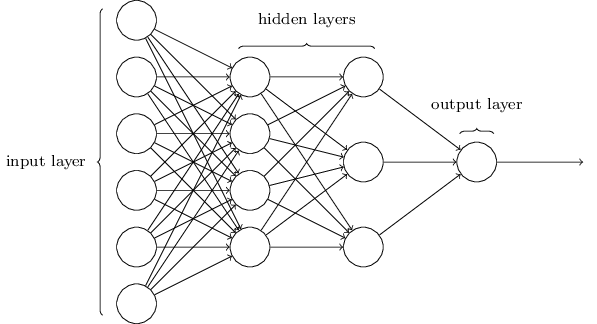
\includegraphics[width=0.7\textwidth]{res/theory-mlp}
        \caption{Beispielhafter Aufbau eines künstlichen, neuronalen Netzwerkes mit zwei verborgenen Schichten, die
            jeweils vier Perzeptronen besizten.\\ Quelle: https://github.com/d-r-e/multilayer-perceptron}
        \label{fig:theory-mlp}
    \end{figure}

    Die einzelnen Gewichte lernen kann dieses Modell indem es die Datenpunkt durch das (untrainierte) Netz
    schickt und die Vorhersage mit der GT vergleicht. In einem Verfahren, was sich Backtracking nennt, werden
    im Grunde die Gewichte, welcher zu einer falschen Entscheidung führten geschwächt, während Gewichte, die
    eine richtige Entscheidung herbeiführen konnten, verstärkt werden. Diese Technik lässt sich durch weitere
    Hyperparameter, welche zum Beispiel die Rate der Verstärkung beeinflussen, optimieren.

   \item \textbf{Linear Regression (LR)} ist eine Regressionsmethode, die versucht, eine Gerade im
    n-dimensionalen Raum zu schaffen, welche die Abstände zu den bekannten Datenpunkten aus $X$ minimiert. Der
    Wert eines neuen Datenpunktes $\hat{x}$ wird nun durch die parametrische Funktion
    \begin{equation}
        f(\hat{x}) = \sum_i w_i\hat{x}_i - \theta
    \end{equation}
    prognostiziert. Um die optimalen Gewichte zu finden, nutzt LR den Mean
    Squared Error (MSE), welcher gegeben ist als
    \begin{equation}
        MSE = \frac{1}{n} \sum_{(x,y) \in X}(y-f(x))^2
    \end{equation}
    und die durchschnittliche, quadrierte Abweichung der Punkte von der Linie beschreibt. Die finalen
    Gewichte sind nun $w = \text{argmin}_{\tilde{w}} MSE$.

   \item \textbf{Ridge (L2)} und \textbf{Lasso (L1)} Regression sind Erweiterungen der LR indem sie einen
    Regularisierungsterm zum MSE hinzufügen, welcher Einfluss auf die optimalen Gewichte hat. Für L2 werden
    die einzelnen Gewichte quadriert und mit einem Hyperparameter $\alpha$\footnote{In der Literatur auch
    häufig $\lambda$ genannt.} multipliziert. Die optimalen Gewichte werden
    damit berechnet: 
    \begin{equation}
        w = \underset{\tilde{w}}{\operatorname{argmin}}\ MSE + \alpha||\tilde{w}||_2^2.
    \end{equation}
    Dadurch werden zu hohe Gewichte und damit Overfitting, was in Kapitel \ref{Section-HyperTuning} weiter
    erklärt wird, bestraft. L1 nutzt die absoluten Werte der Gewichte:
    \begin{equation}
        w = \underset{\tilde{w}}{\operatorname{argmin}}\ MSE + \alpha||\tilde{w}||_1.
    \end{equation}
    Während L2 aufgrund der Natur quadratischer Funktionen den Wert von $\alpha$ nur asymptotisch gegen $0$ gehen
    lassen kann, kann L1 diesen komplett auf $0$ setzen. Damit kann einfacher mit Dimensionen umgegangen werden,
    die nur wenig Einfluss auf das Endergebnis haben.

\end{itemize}

Das korrekte Setzen der Hyperparameter gehört zu dem Fachbereich des Fine Tunings von Modellen und kann
 gravierende Effekte auf das Endergebnis haben. Methoden um diese Aufgabe anzugehen, werden in den
 nächsten Kapiteln beschrieben.


\section{Evaluation und Metriken}

Um einschätzen zu können, wie gut ein Modell mit gegebenen Hyperparametern und ausgewählten Daten das Problem
 löst, wird eine Metrik benötigt. Eine solche ist definiert als Funktion, welche die wahren und die
 prognostizierten Werte annimmt und einen einzigen Wert\footnote{typischerweise zwischen 0 und 1} als
 Indikator, wie gut in einer gewissen Disziplin abgeschnitten wurde, zurückgibt. Die meisten Metriken,
 die in dieser Arbeit verwendet werden, können aus der Konfusionsmatrix berechnet werden. Für ein binäres
 Klassifikationsproblem hat sie den folgenden Aufbau:

\renewcommand{\arraystretch}{1.5}
\begin{table}[h]
    \centering
    \begin{tabular}{c c c c}
        & & \multicolumn{2}{c}{Echtes Label} \\
        \cline{3-4}
        & & 1 & 0 \\
        \hline
        \multirow{2}{10em}{Ausgabe des Modells} & 1 & \textbf{TP} & \textbf{FP} \\
        \cline{2-4}
        & 0 & \textbf{FN} & \textbf{TN} \\
        \hline
    \end{tabular}
\end{table}

% \begin{center}
%     \hspace{3.1cm}
%     \begin{tabular}{ c c | c c | }
%         & & \multicolumn{2}{c}{Echtes Label} \\
%         & & 1 & 0 \\ 
%         \hline
%         \multirow{2}{10em}{Ausgabe des Modells} & 1 & \ TP & \ FP \\  
%         & 0 & \ FN & \ TN \\
%         \hline  
%     \end{tabular}
% \end{center}

Auf der Diagonalen steht TP (True Positive) für die Menge an positiven Fällen, die auch als solche erkannt
 wurden, und TN (True Negative) für alle negative Fälle, die ebenfalls richtig vom Modell erkannt wurden.
 Die anderen Werte stehen für keine Übereinstimmung der Werte; FN (False Negative) steht für fälschlicherweise
 als negativ klassifizierte Datenpunkte und FP (False Positive) für welche, an denen das Modell ohne Grund
 positiv angeschlagen hat. Tabelle \ref{tab:theory-metrics} zeigt ausgewählte Metriken, die in dieser Arbeit benutzt werden und was sie
 in diesem Kontext bedeuten.

\renewcommand{\arraystretch}{1.5}
\begin{table}
    \begin{tabular}{ m{6em} m{9em} m{14em} }
        Metrik & Berechnung & Bedeutung \\
        \hline
        Accuracy              & $\frac{TP+TN}{TP+TN+FP+FN}$ & Wie oft lag der Algorithmus richtig? \\
        Sensitivität (auch Recall) & $\frac{TP}{TP+FN}$          & Wie gut wurden echte Lecks erkannt? \\
        Specificity           & $\frac{TN}{TN+FP}$          & Wie gut wurde 'alles ok' erkannt? \\
        Precision             & $\frac{TP}{TP+FP}$          & Wie viele erkannte Lecks waren auch wirklich Lecks? \\
        Detection\ \ \ \ \ \ Time & Mittelwert vom Auftreten eines Lecks bis zur Erkennung & Wie viele Zeiteinheiten dauerte es bis zum Erkennen?
    \end{tabular}
    \caption{Definitionen und Bedeutungen wichtiger Metriken.}
    \label{tab:theory-metrics}
\end{table}

Hierbei ist wichtig anzumerken, dass auch wenn die Accuracy alle Werte der Konfusionsmatrix in die Bewertung
 mit einfließen lässt, diese nur als grobe Einschätzung genutzt werden sollte, da sie im Vergleich zu den anderen
 Metriken keine Begründung liefert, wie die anderen Metriken. Zudem kann sie auf unbalancierten Datensätzen ein
 falsches Bild vermitteln\footnote{Gibt ein Modell konstant nur Label 0 aus, so ist die Accuracy auf einem
 Datensatz, welches nur ganz wenige Punkte mit Label 1 besitzt, bei annährend 100\%}.

Um die Metriken erheben zu können, muss man jedoch definieren, welche Datenpunkte hierfür genutzt werden
 und welche nicht. Das nächste Kapitel gibt Aufschluss darüber, wie dies bewerkstelligt werden kann.


\section{Hyperparameter Tuning \label{Section-HyperTuning}}

Das Ergebnis eines Machine Learning Modells hängt stark von den gewählten Hyperparametern ab. Diese zu
 optimieren gehört zu den Kernaufgaben des Modellierungsprozesses, für die jedoch eine Verlässliche Aussage
 der Metriken wichtig ist. Man sollte davon absehen, auf den gleichen Daten zu testen, auf denen man bereits
 trainiert hat. Dabei kann es nämlich unbemerkt zu Overfitting kommen, was bedeutet, dass das Modell nicht
 genug generalisiert, sondern die Eigenheiten des Datensatzes, wie zum Beispiel Rauschen, lernt. Dadurch
 funktioniert es schlechter auf nicht gesehenen Daten. Weiter sind Metriken nicht mehr so aussagekräftig,
 wenn nur bereits Bekanntes abgefragt wird\footnote{Mit $k=1$ hätte kNN einen Fehler von $0$, falls auf den
 gleichen Daten getestet und trainiert wird.}. Die Test- und Trainingsdaten sollten also disjunkt sein.

\subsection*{Train-Test-Split}

Beim Train-Test-Split wird die Datenmenge in zwei Gruppen aufgeteilt: Das Train-Set und das Test-Set.
 Typischerweise beträgt die größe des Test-Sets zwischen 20\% und 33\% der gesamten Daten. Da bei diesem Split
 auf neuen Daten getestet wird, zwingt es einen dazu, das Modell so zu gestalten, dass es gut generalisieren
 kann. Bei einer unglücklichen Wahl des Test-Sets, wenn beispielsweise keine Punkte einer Klasse im Test-Set sind,
 kann es jedoch immer noch passieren, dass die Metriken einen falschen Eindruck hinterlassen.

\subsection*{Cross-Validation}

Die Lösung dieses Problems ist das wiederholte Anwenden eines Train-Test-Splits. Bei der sogenannten
 k-Fold Cross-Validation wird der Datensatz in k gleich große Mengen unterteilt. Mit dieser Aufteilung
 wird dann k-Mal der Prozess des Trainierens und Testens gestartet, wobei jedes mal ein anderes der k Sets als
 Test-Set gewählt wird. Abbildung \ref{fig:theory-cv} visualisiert dieses Vorgehen. Die Ergebnisse der k Durchläufe
 werden anschließend gemittelt und zeigen damit eine weitaus robustere Einschätzung der Güte auf. Das k liegt hier
 typischerweise\footnote{Es gibt einen Spezialfall, indem k gleich der größe des Datensatzes ist. Eine solche
 Einstellung nennt sich Leave-One-Out Cross-Validation, bei welcher immer auf allen Datenpunkten mit Ausnahme
 eines einzigen Punktes trainiert wird. Dies ist jedoch nicht Thema dieser Arbeit.} zwischen 3 und 10.

\begin{figure}
    \centering
    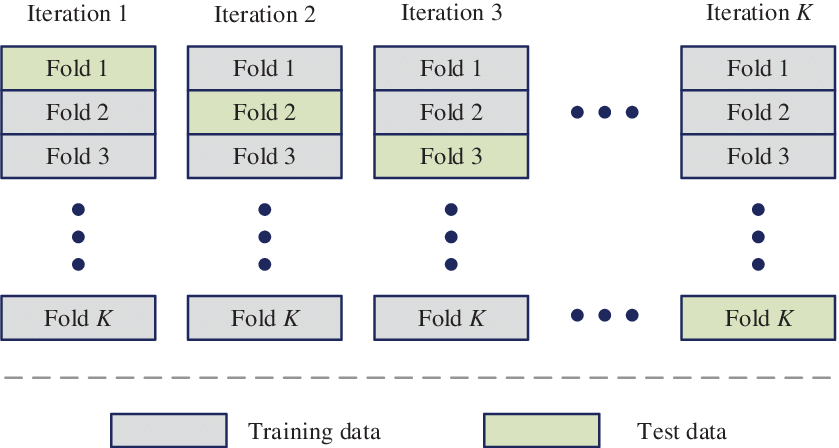
\includegraphics[width=0.7\textwidth]{res/theory-cv}
    \caption{Aufbau einer k-Fold Cross Validation.\\ Quelle: https://www.researchgate.net/figure/K-fold-cross-validation-method\_fig2\_331209203}
    \label{fig:theory-cv}
\end{figure}

\subsection*{Grid-Search}

Mit dieser Technik können nun verlässlich die Hyperparameter analysiert werden. Mit der Methode des Exhaustive
 Grid-Search lassen sich alle Hyperparameter testen, indem das kartesisches Produkt der möglichen Einstellungen
 gebildet und auf allen Kombinationen mittels Cross-Validation trainiert und getestet wird. So wird für kNN einmal
 mit uniformer Gewichtung der Nachbarn jede Einstellung für k getestet und einmal mit distanzbedingter Gewichtung.
 Das Ergebnis zeigt nun die optimale Einstellung für die Gewichtsfunktion und das k an. Ebenso können weitere
 Relationen ausgelesen werden; Beispielsweise könnte für ein höheres k die distanzbedingte Gewichtung besser
 funktionieren, für kleinere k jedoch eher die uniforme Gewichtung.
